\documentclass[../main.tex]{subfiles}
\begin{document}

\subsection{Web application for simulating spikes}
I have created an application that can be used to generate surrogate spike sequences. The app generates spike sequences using the methods described in section -. The application can be found at {\tt https://shiny.maths.nottingham.ac.uk/pmxjp8/SimSpikes/}. Once opened you will see a panel explaining how to use the app and a sidebar with a number of inputs. The inputs are as follows:

\begin{itemize}
	\item ISI distribution,
	\item ISI parameter value,
	\item end time,
	\item refractory period,
	\item intensity function,
	\item how many sequences.
\end{itemize}

Once the desired inputs have been entered you press the {get spikes} button. This will generate the specified number of spike sequences. The main panel will be updated with a plot of the intensity function and underneath the plot there is the rastor plot of the generated spike sequences (with a maximum of 20 shown). Furthermore, underneath the plot the first generated sequence is written. Click the toggle button to swap between instructions and results window if needed. Pressing the download button with create a folder on your local computer, once extracted the folder will contain two files: a text document containing the inputs and a {.csv} file containing each spike sequence as a new column. 

\subsubsection{Example of using the app}
I will give two examples of using the application, one to generate spikes from an oscillating intensity and one from a step change. In the first example I set the parameters as follows: ISI distribution to Gamma, ISI parameter to 32, end time to 40, refractory period to 0, intensity function to $\cos \left( t/2.3 \right) +1.2$ and the number of sequences to 1. Pressing get spikes gives the pane show in \ref{fig: SimSpikes example}A. Where the intensity is plotted with the  spike sequence shown below by the black points. Furthermore, the sequence is written explicitly below the plot. 

For the step change I decided to change the parameters to as follows: ISI distribution to Weibull, ISI parameter to 7, end time to 40, refractory period to 0, intensity function to $c\left(t\left[t < 20 \right]*0 +1.6, t\left[t > 20 \right]*0 +0.5  \right)$ and the number of sequences to 25. The input for the intensity may look confusing, however this is the format required for R to understand the step function. The intensity function is generated by applying the input provided to the vector $t$, which is the sequence starting from $0$ to the inputted end time in 8000 equal steps. Thus, in the case of the step function we split the $t$ vector into two for values less than 20 by $t\left[t < 20 \right]$ and similarly for greater than 20. Then to get the constant intensity we multiply this vector by $0$ and add the value we want the intensity to be. In our case we set the intensity to 1.6 between 0 and 20 and 0.5 between 20 and 40. Then to join the two vectors back together we use $c()$ which is used by R to concatenate the vectors together. This method can easily be used in combination with functions to create more complicated intensity functions as inputs. For example $\cos \left( t\left[t < 20 \right] \right) + 1.4$ sets the intensity to be $cos(t) +1.4$ between the times 0 and 20. 

	Clicking the get spikes button is show in \ref{fig: SimSpikes example}B. We see that since we increased the number of sequences to generate there are more spike sequences shown as rastors underneath the plot of the intensity function, however only one sequence is still printed below the plot. Clicking the download button creates a new folder on your local computer called SimSpikes. Opening the folder you are greated by two files one called {details.txt} and another called {spikes.csv}. Figure \ref{fig: SimSpikes Download}(A) shows the contents for {details.txt}, which included all the inputs used to generate the spike sequences. This is useful incase when using the simulated spikes at a later date you have forgotten the inputs used to them. Figure \ref{fig: SimSpikes Download}(A) is a screenshot of the {spikes.csv} in Excel, you can see that each spike sequence is stored as a column in the table. Each column contains the generate spike sequence adjoined with the simulation end time. Since is generates sequence will not have the same number of spikes, columns contain NA values after the sequence.


\begin{figure}
	\begin{subfloat}[]{
	\includegraphics[width = 0.5\linewidth]{SimSpikes_2}}
	\end{subfloat}
	\begin{subfloat}[]{
	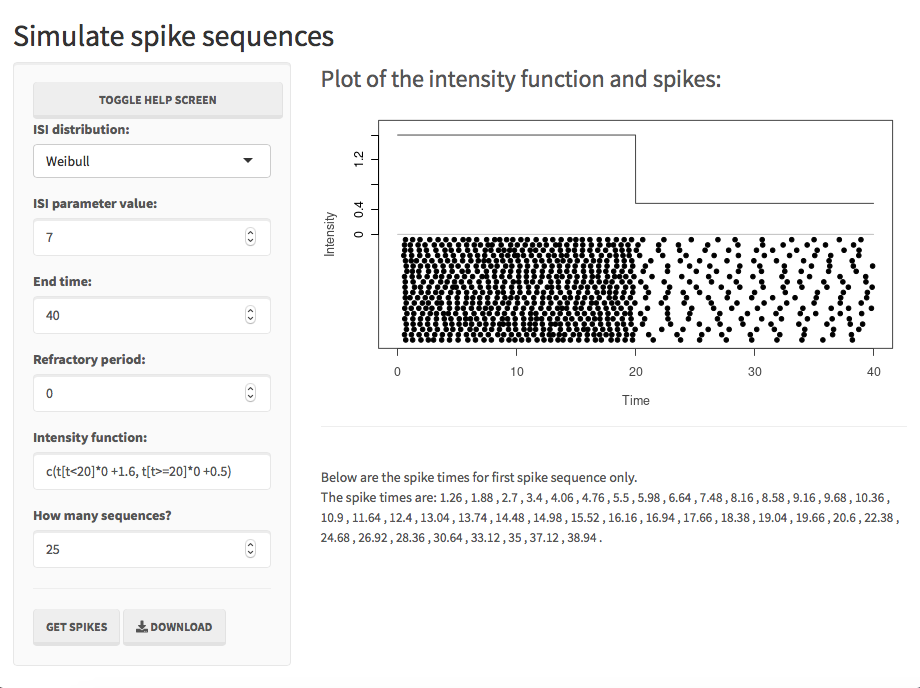
\includegraphics[width = 0.5\linewidth]{SimSpikes_3}}
	\end{subfloat}	
		\caption{Examples of generated spike sequences using {SimSpikes}. }
\label{fig: SimSpikes example}
\end{figure}

\begin{figure}
	\begin{subfloat}[]{
	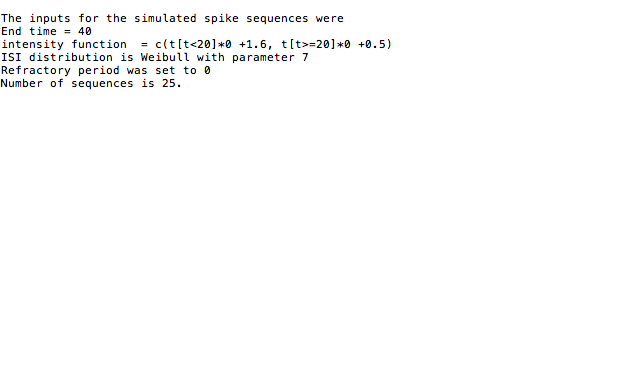
\includegraphics[width = 0.5\linewidth]{SimSpikes_5}}
	\end{subfloat}
	\begin{subfloat}[]{
	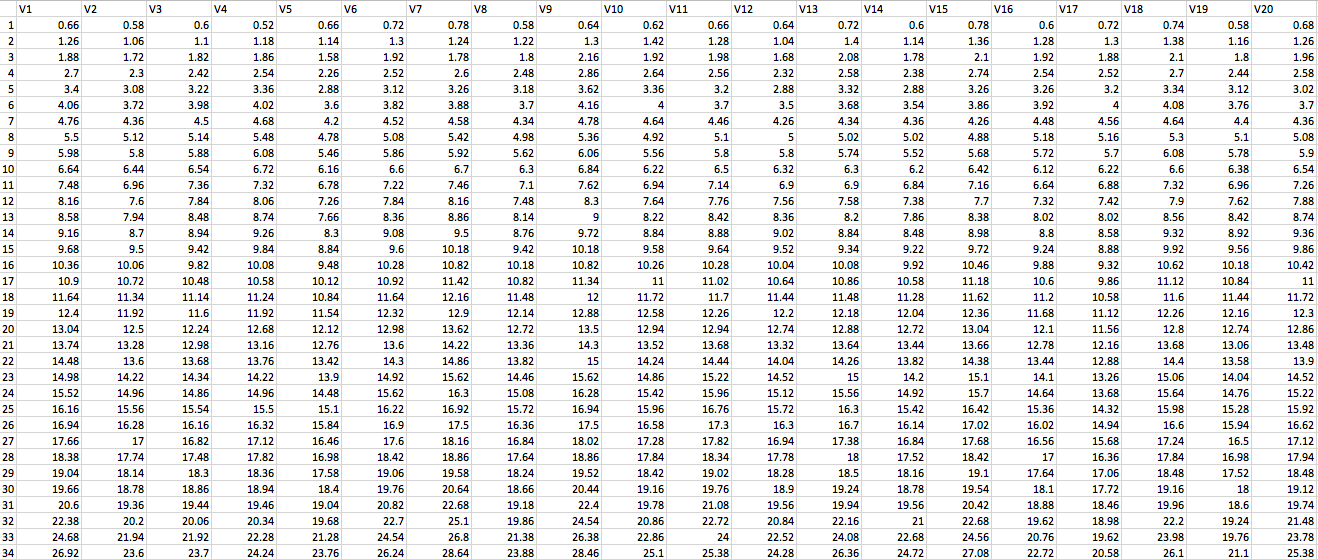
\includegraphics[width = 0.5\linewidth]{SimSpikes_6}}
	\end{subfloat}	
		\caption{Images of the files downloaded from the step change intensity function {SimSpikes}. }
\label{fig: SimSpikes Download}
\end{figure}


\subsection{Web application for viewing/analysing raw data}
I have created an application that can be used to view the raw time series data and then  threshold to retrieve spike sequences. The application can be found at {\tt https://shiny.maths.nottingham.ac.uk/pmxjp8/ViewData/}. The application was created with the aim at easily viewing the raw time series data with a user-friendly method of thresholding the data to calculate spike times. Once the application is opened you are greeted with a panel explaining how the application works and a sidebar where inputs can be altered. To begin you need to input the raw data, which needs to be formatted in a `.csv' file such that the first column corresponds to the time indexing and each following column corresponds to the calcium concentration at the times for a single cell. If the uploaded file has missing data the upload will fail and the user is prompted with the reason. 

Once the upload has been successful a plot of calcium concentration against time will appear for the first cell, with an option on the sidebar to toggle between the different cells. By changing inputs on the sidebar the user can threshold the data which can be seen on the time series plot, further to this a new plot showing the ISIs will appear and the spike times written below. Once some of the data has been analysed the user can download the spikes and corresponding threshold details by clicking the download button which will save the results on the users home computer, which can be reloaded into the app at a later date.   

\subsubsection{Example of using the app}
A guide to using the app appears on loading the webpage. A run through of an example is provided here where we upload some data and retrieve spike times.

Firstly, we click on the `INPUT DATA' button, and a pop up window appears. We then click browse and choose the file `data.csv' from our local PC. Once the file is successfully uploaded we click `ok' to finish the upload. If we have already uploaded, analysed and downloaded from the application we can also upload 'spike details' using the second upload box, which will then present the details from the previously analysed data. 

Returning to just uploading data once we have clicked `ok', we are shown the plot of calcium concentration against time for cell 1 - as seen in figure \ref{}. On the sidebar under cell number we can toggle which cell's information we look at, the current cell number can be seen in this section of the sidebar and is also printed above the plot along with the number of cells that the data contains. The x and y axes for the concentration plot can be changed by unchecking the default axes buttons on the sidebar where you are then prompted to enter the range of values you want to view. This function is useful to zoom in on the plot for a better view. 

Now we will consider thresholding the data for cell 1. In the sidebar there is section labelled 'Thresholding', under this section we can tell the application the heights at which we wish to threshold the data, as well as removing transient sections or removing linear trends in the data. We may want to remove transient regions since after applying a stimulus there is often a time window where the calcium concentration is non-stationary and we only want to consider spikes that are in a stationary regime. Furthermore, the user may want to remove linear trends as they could be caused by experimental effects such as de-sensitisation of the tracer placed in the cell and doesn't reflect the true nature of the calcium spiking rate.

\begin{figure}[t]
	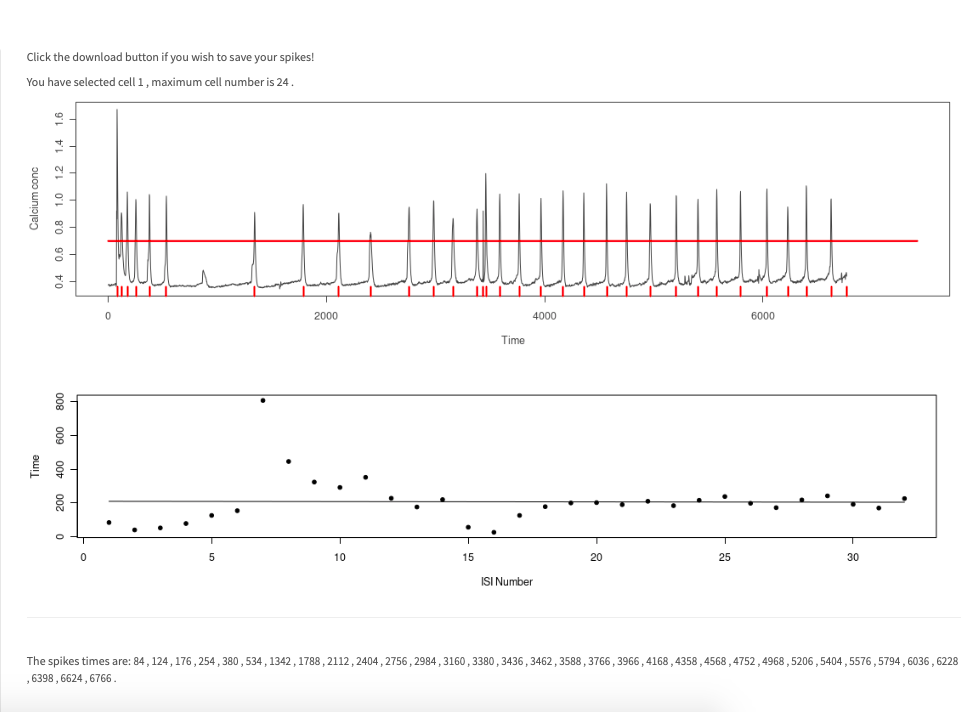
\includegraphics[width=\linewidth]{ViewData}
	\caption{Print-screen of main pain of ViewData app where the threshold input has been updated to be $0.7$. }
	\label{fig: ViewData}
\end{figure}

Looking at cell one it seems reasonable to threshold the spikes at the concentration value 0.7. We enter the value into the `Threshold at?' in the sidebar and the application updates and shows figure \ref{fig: ViewData}. We see that the threshold line shows up on the concentration plot as a red line, and the red ticks on the x-axis shows the spike times. A new plot is produced under the concentration plot, which shows the ISI times for the thresholded data, which can aid in seeing any patterns in the spikes that are harder to visualise from the concentration plot. For example, if the ISI times slowly decreased this would be easier to see in ISIs rather than the raw spike times Furthermore, in the ISI plot we fit the linear line of best fit to show the linear trends in the ISIs. Then underneath the ISI plot, the spike times are explicitly written, which can makes the spikes easily accessible via a copy and paste rather than having to download the data for all the cells. 

Consider again the plot in figure \cite{fig: ViewData}, if we look between times 800 and 1000 we see a small spike in the calcium concentration that we may want to include as a spike time, however if we lowered the threshold time we may lose some of the other spikes (i.e at the beginning when the concentration is higher then the little bump). So, to include this value we can enter multiple threshold values by entering `0.7,0.45,0.7,800,1000' into the threshold at? box. This tells the app that between times 0 and 800 you want to threshold at 0.7, between 800 and 1000 threshold at 0.45 and threshold at 0.7 for time greater than 1000. In figure \ref{fig: ViewData2} we see the red line has updated for our new threshold value and a new red tick is produced the new spike we have included.  

\begin{figure}[t]
	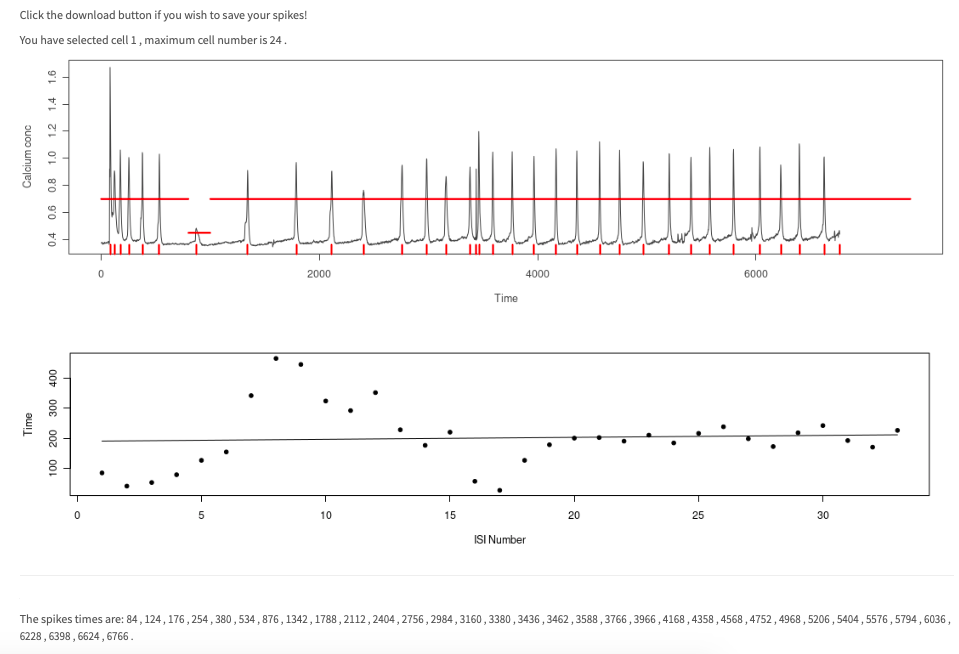
\includegraphics[width=\linewidth]{ViewData2}
	\caption{Print screen of App where threshold has been updated to `0.7,0.45,0.7,800,1000'.}
	\label{fig: ViewData2}
\end{figure}


Continuing with cell one the data comes from a step change experiment and we may want to remove the transient sections at the start and middle of the experiment. By checking the transient period box in the sidebar we are prompted to enter the transient regions at either the start, middle or end of the experiment. Looking at cell one we choose to transient periods to be between 0 and 200 at the start and between 3300 and 3500 in the middle. In figure \ref{fig: ViewData3} we see the affect of changing these values. In the concentration plot red boxed now appear over the inputted transient periods. Notice that the red ticks now occur for spikes outside of the red boxes except for the first spike outside of these regions this is because these first spikes are taken as the start time of the sections. For example in the first section we say the region 0s to 200s is transient and the next spike outside this region previously occurred at 254s. Since removing transient regions is $done becuase$ we want to consider stationary spikes, the region between the cutoff and the next spike is dependent on the cutoff, however by removing the first spike and setting the first spike time as time zero all the following ISI are true ISI. In the ISI plot the plot is now split into two windows one for the spikes before the middle transient period and one for afterwards, with each having its own linear trend line. 

\begin{figure}[t]
	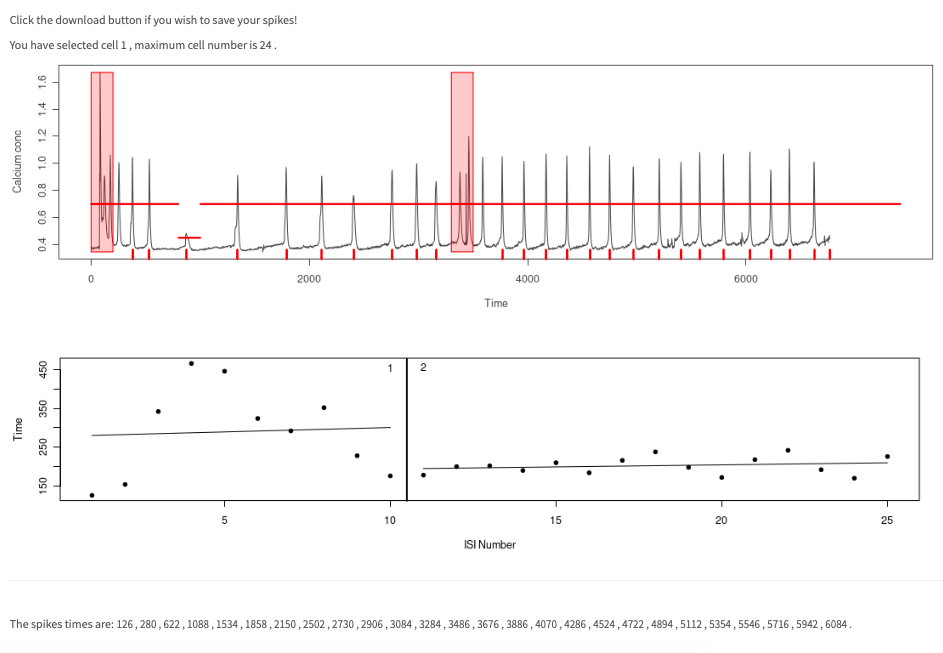
\includegraphics[width=\linewidth]{ViewData3}
	\caption{Main Panel where we remove two transient regions. The first region between 0s and 200s. The second interval is between 3300s and 3500s.}
	\label{fig: ViewData3}
\end{figure}

Considering the relationships in the ISI plot both appear to have a minimal positive trend, we can remove these linear trends by checking the `Remove linear trends?' box. In figure \ref{fig: ViewData4} we have removed the linear trends we see this has no affect on the concentration plot but now in the ISI plot both linear fits are flat showing there are no linear trends in the adjusted data. 

\begin{figure}[t]
	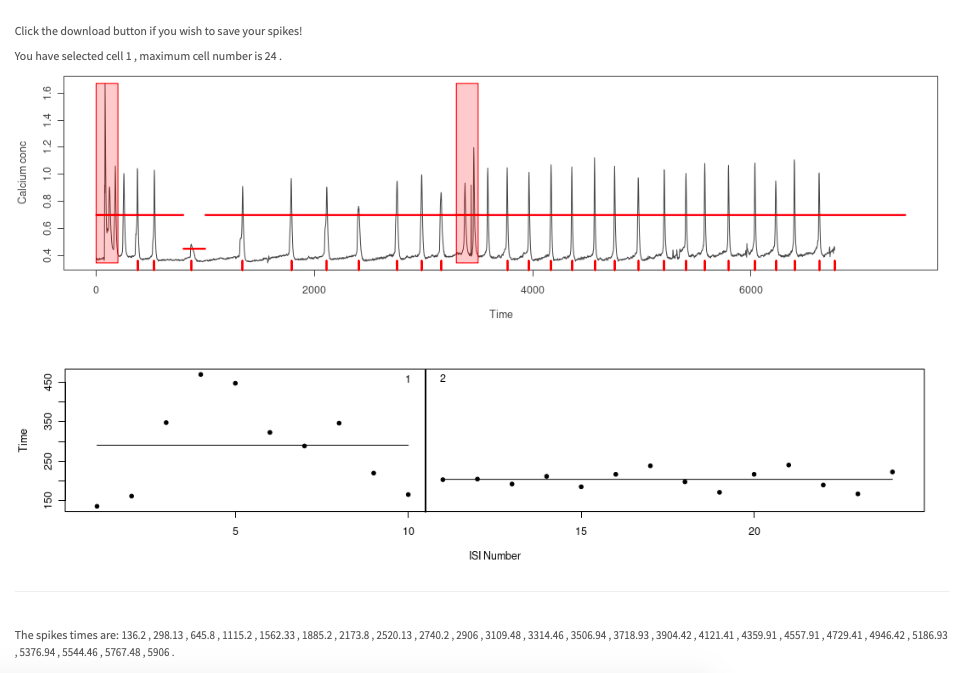
\includegraphics[width=\linewidth]{ViewData4}
	\caption{Main panel where linear trends are removed.}
	\label{fig: ViewData4}
\end{figure}

We have now decided that we have successfully got the spikes for cell one and we wish to download the spikes for later use. Clicking on the `Download' button will either save to your download folder automatically or prompt the user for a download. In the downloaded folder there will be three files. The first file entitled `Details.txt' stores the data file from which we analysed the raw data in this case 'Data.csv'. The second file is called `spikes.csv' which stores the resultant spike sequences for each cell as a column in the file, see figure \ref{}. Cells which have not been thresholded will have a column of NA's in the file. The third file `store.csv', contains the threshold details for each cell in the analysis. This is the file that can be uploaded at the start of the program along with the raw data to show the threshold details used, or can be used as a basis to update the threshold if mistakes were initially made. 








\end{document}
